%% ARXIV-ONLY fork of sections/intro.tex — arxiv.tex inputs this file;
%% main.tex keeps sections/intro.tex untouched (the POPL submission is
%% frozen). Deliberately short: more than the abstract, less than the
%% paper; \Cref{fig:planes} carries the two-plane structure the prose
%% no longer narrates. Cherry-pick by diffing against sections/intro.tex.

\section{Introduction}
\label{sec:intro}

To answer a question about a program, move the program to where the
question is decidable. A C program's reachability question becomes a
bit-vector model-checking problem; a Python function's assertion becomes
a linear-arithmetic query; a chemical reaction network's coverability
question becomes an SMT unrolling. Every such move is a translation, and
every translation is a place to be wrong. The classical responses are to
\emph{prove} the translator once and for all
\citep{leroy2009compcert,kumar2014cakeml}, or to \emph{validate} each of
its runs \citep{pnueli1998tv,necula2000tv,lopes2021alive2}. Both are
statements about a single edge.\repofootnote

This paper is about the \emph{graph}: several source languages, a few
solver-facing targets, more than one way to get from here to there ---
and, crucially, edges of \emph{honestly different} trustworthiness. A
rule-for-rule logic translator is foreseeable from its specification; an
optimizing C compiler is only pinned; two translators derived
independently from a prose manual and a formal model are neither proved
--- but their independence is itself a resource. A theory of the graph
must let each edge say what it actually guarantees, compose those
statements honestly, and let weak edges corroborate one another into
strong routes. Its stance is that of distributed systems: a translator
is a component that fails, and failure is \emph{contained} --- by
declared loss, decidable checks, and independent routes --- not
prevented by universal proof.

\begin{figure}
\centering
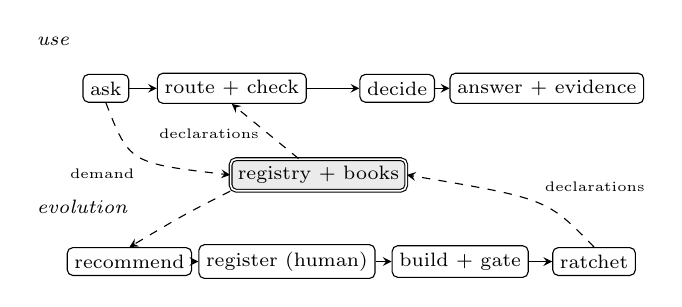
\begin{tikzpicture}[x=1cm, y=1cm,
  stg/.style={draw, rounded corners=2pt, inner sep=2.6pt, font=\scriptsize},
  flow/.style={->, >=stealth},
  data/.style={->, >=stealth, dashed},
  planelbl/.style={font=\scriptsize\itshape, anchor=west}]
\node[planelbl] at (-0.4, 1.0) {use};
\node[stg] (q)  at (0.6, 0.4)  {ask};
\node[stg] (r)  at (2.2, 0.4)  {route + check};
\node[stg] (d)  at (4.3, 0.4)  {decide};
\node[stg] (a)  at (6.2, 0.4)  {answer + evidence};
\draw[flow] (q) -- (r); \draw[flow] (r) -- (d); \draw[flow] (d) -- (a);
\node[stg, double, fill=black!8] (reg) at (3.3, -0.7) {registry + books};
\draw[data] (reg) -- (r.south) node[pos=0.45, left, font=\tiny] {declarations};
\draw[data] (q.south) .. controls (0.9, -0.55) .. (reg.west)
  node[pos=0.55, below left, font=\tiny] {demand};
\node[planelbl] at (-0.4, -1.1) {evolution};
\node[stg] (rec) at (0.9, -1.8)  {recommend};
\node[stg] (hu)  at (2.9, -1.8)  {register (human)};
\node[stg] (bg)  at (5.1, -1.8)  {build + gate};
\node[stg] (ra)  at (6.8, -1.8)  {ratchet};
\draw[flow] (rec) -- (hu); \draw[flow] (hu) -- (bg); \draw[flow] (bg) -- (ra);
\draw[data] (reg.south west) .. controls (1.6, -1.2) .. (rec.north);
\draw[data] (ra.north) .. controls (6.2, -1.0) .. (reg.east)
  node[pos=0.5, above right, font=\tiny] {declarations};
\end{tikzpicture}
\caption{The two planes, meeting in one data structure. The use plane
reads the registry's declarations and produces evidence-carrying
answers; the evolution plane turns recorded demand into new
declarations, gated and ratcheted, with registration a human act.
\emph{Answers never write; growth never answers.}}
\label{fig:planes}
\end{figure}

\paragraph{Two directions, two planes}
This work is as much an experiment about \emph{who can build and use}
such a system as about the system itself, and its two directions are
the platform's two planes (\Cref{fig:planes}). On the \emph{use} plane,
LLMs are \emph{supported}: the intended player is an LLM that chooses
questions and routes but can take no unchecked step --- every move is
deterministic, graded, cross-checked, and, for witness-carrying
answers, self-certifying at the source (a first controlled experiment:
\S\ref{sec:eval-player}). On the \emph{evolution} plane, LLMs are
\emph{utilized}: every pair was implemented by an independent LLM agent
from a one-page brief, largely unsupervised, with the architecture's
cross-checks as the only semantic gate (\S\ref{sec:bugs} reports what
the gate caught) --- and the plane is instrumented end to end:
unanswerable questions are diagnosed and recorded as demand, pairs are
\emph{recommended by evidence} before a human registers them, and the
ratchet (\Cref{prop:ratchet}) keeps every prior verdict standing
(\S\ref{sec:books}). Run indefinitely, this loop is a semi-algorithm
for answerability: in the limit it reaches every \emph{reducibly
decidable} question, at fidelity that only rises --- and it is not an
oracle: undecidability, the adequacy floor, and the finite supply of
independent semantic anchors stand at every graph size
(\Cref{sec:overview,sec:conclusion}).

\paragraph{Provenance disclaimer}
All of \hg\ --- framework, interpreters, pairs, solver plumbing,
evaluation harness, Lean mechanization --- is LLM-generated code
(Claude Opus and Claude Fable agents), and most of this paper's text is
LLM-generated too; no human reviewed either for semantic correctness.
The human contribution is the architecture: the calculus, the
contracts, and the decisions about what to build and claim. Every
quantitative claim in \Cref{sec:evaluation} regenerates from the
artifact by one script, and the mechanization's axiom audit re-runs at
every build --- the reader need not trust the writers, human or
otherwise, beyond what the thesis itself requires.

\paragraph{This paper}
The unit is the \emph{pair} (\Cref{sec:calculus}): two languages, a
pure translator, shared pure interpreters, and a pure
\emph{target-to-source interpreter} carrying target behaviors back to
source vocabulary. These close a commuting square that is
\emph{directional} --- exactness is the identity-embedding special case
of over-approximation --- and \emph{decidable per program}: run both
sides, compare under the declared projection, and a failure names its
step and observable. Squares paste (under a one-line congruence
condition on what carry-backs may read), and composition is told once:
a pair's \emph{contract} --- assurance class, direction, kept
observables, measured cost --- composes along a route by the
componentwise meet, the weakest hop on every axis at once
(\Cref{sec:fidelity}). Two mechanisms move trust where the meet says it
cannot go --- per-run re-establishment by inline checking, and
corroboration by independently derived branches whose declared
semantic artifacts are disjoint --- and one asymmetry caps the story:
existential answers are self-certifying by replay
(\Cref{thm:existential}), while universal answers are exactly where
grades, branches, and certificates earn their cost
(\Cref{thm:universal}). \Cref{sec:instantiation} describes the
platform --- 13 languages, 15 registered pairs (13 in the evaluated
snapshot), two reasoning hubs --- \Cref{sec:economy} its economy and
books, and \Cref{sec:evaluation} measures both.

\paragraph{Contributions}
\begin{itemize}
\item A calculus of directional, fidelity-graded translation pairs:
  per-program decidable squares with localization, pasting under an
  explicit support condition, exactness as the identity-embedding case
  (\Cref{prop:exactid}), and universal transfer across
  over-approximation (\Cref{prop:lax}).
\item The contract algebra: composition as one componentwise meet
  across assurance, direction, loss, and cost --- mechanized in Lean~4
  with the rest of the compositional core, lax telescope included
  (\S\ref{sec:mech}).
\item The existential/universal asymmetry as an architectural
  principle, with its end-to-end theorems (\S\ref{sec:endtoend}).
\item The two-plane architecture and its economy: demand books,
  evidence-backed recommendation, human-valved registration, and the
  ratchet --- the untrusted-generator stance extended from building
  pairs to choosing them (\S\ref{sec:books}).
\item A measured, LLM-built instantiation: conjoined coverage, dual
  ISA branches with disjoint decision stacks, a compliance-derived
  benchmark, witness replay, certified unreachability at up-to-megabyte
  scale under a formally verified checker, gate escape rates, a first
  LLM-player experiment, and the defects caught
  (\Cref{sec:instantiation,sec:evaluation}).
\end{itemize}

This document is a dated capability snapshot (July 2026) of a system
whose coverage ratchets monotonically by construction; every number in
\Cref{sec:evaluation} regenerates from the artifact, and the appendix
--- detailed proofs and the construct-inventory catalog --- follows the
bibliography.
